
訪問共享數據而不進行訪問同步(通常是互斥或原子訪問)的程序都會出現未定義行為,這通常稱為數據競爭。這看起來很簡單,至少在理論上是這樣,而我們的例子太簡單了,只有一個變量在線程之間共享。但在現實中,併發不僅僅是鎖定共享變量那麼簡單。

\subsubsubsection{5.5.1\hspace{0.2cm}順序的必要性}

來看一下\textbf{生產者-消費者}的例子。假設有兩個線程:第一個線程(生產者)通過構造對象準備一些數據;第二個線程,即消費者,處理數據(處理每個對象)。簡單起見,假設有一個很大內存緩衝區,沒有初始化,生產者線程在緩衝區中構造新的對象,就如同數組元素一樣:

\begin{lstlisting}[style=styleCXX]
size_t N; // Count of initialized objects
T* buffer; // Only [0]…[N-1] are initialized
\end{lstlisting}

為了生成(構造)一個對象,生產者線程通過\texttt{new}操作符對數組的每個元素進行構造,從\texttt{N==0}開始:

\begin{lstlisting}[style=styleCXX]
new (buffer + N) T( … arguments … );
\end{lstlisting}

現在,初始化數組\texttt{buffer[N]},並可用於消費者線程。生產者通過推進計數器\texttt{N}來表示,然後繼續初始化下一個對象:

\begin{lstlisting}[style=styleCXX]
++N;
\end{lstlisting}

當\texttt{i}大於\texttt{N}時,消費者線程不能訪問數組元素\texttt{buffer[i]}

\begin{lstlisting}[style=styleCXX]
for (size_t i = 0; keep_consuming(); ++i) {
	while (N <= i) {}; // Wait for the i-th element
	consume(buffer[i]);
}
\end{lstlisting}

忽略內存耗盡的問題,並假設緩衝區足夠大。此外,現在不關心終止條件(消費者如何知道可以繼續消費?)。目前,感興趣的是生產者-消費者信號交換協議,消費者如何在沒有任何競爭的情況下訪問數據?

規則對共享數據的任何訪問都必須受到保護。顯然,\texttt{N}是一個共享變量,所以對它的訪問需要更多的注意:

\begin{lstlisting}[style=styleCXX]
size_t N; // Count of initialized objects
std::mutex mN; // Mutex to guard N
… Producer …
{
	std::lock_guard l(mN);
	++N;
}
… Consumer …
{
	size_t n;
	do {
		std::lock_guard l(mN);
		n = N;
	} while (n <= i);
}
\end{lstlisting}

這就足夠了嗎?在程序中出現了更多的共享數據。數組\texttt{T}在兩個線程之間共享,線程需要訪問每個元素。如果鎖定整個數組,因為兩個線程中總有一個需要等待解鎖,那就和單線程的實現沒區別了。根據經驗,寫過多線程代碼的開發者都知道,不需要鎖定數組,只需要鎖定計數器即可,因為這個數組不會併發訪問。首先,生產者在計數器遞增之前訪問這個數組。然後,在計數器增加後,消費者才會訪問這個數組,這些都是已知情況。但本書的目的是讓你理解程序為什麼會這樣做。那麼問題來了,為什麼鎖上計數器就足夠了?是什麼保證程序真的按照期望的順序執行呢?

現在這個簡單的例子,也變得不那簡單了。無效的保護消費者使用計數器的代碼如下所示:

\begin{lstlisting}[style=styleCXX]
std::lock_guard l(mN);
while (N <= i) {};
\end{lstlisting}

這是一個有死鎖寫法。當使用者獲得了鎖,就會等待元素\texttt{i}初始化。生產者無法進行操作,只能等待解鎖,然後才能增加計數器\texttt{N}。兩個線程現在都在永遠等待。如果只是為計數器使用原子變量,代碼就會簡單很多:

\begin{lstlisting}[style=styleCXX]
std::atomic<size_t> N; // Count of initialized objects
… Producer …
{
	++N; // Atomic, no need for locks
}
… Consumer …
{
	while (N <= i) {};
}
\end{lstlisting}

現在,消費者對計數器\texttt{N}的讀取是原子的,但在兩次讀取之間,生產者沒有阻塞,可以繼續工作。這種實現併發的方法稱為\textbf{無鎖}(它不使用任何鎖),我們將在稍後討論這種方式。現在的問題是:是否能夠保證生產者和消費者不在同時訪問同一個\texttt{buffer[i]}?

\subsubsubsection{5.5.2\hspace{0.2cm}內存序和內存柵欄}

僅僅能夠安全地訪問共享變量,還不足以應對併發程序,還要能夠推理出事件發生的順序。在生產者和消費者的例子中,整個程序基於一個假設:可以保證第\texttt{N}個數組元素的構造時,可以將計數器增加到\texttt{N + 1},並且消費者線程訪問第\texttt{N}個元素也是按這個順序進行。

但當意識到需要處理的不僅僅是多個線程,而是多個處理器同時執行這些線程時,問題就會變得更加複雜。這裡的關鍵是\textbf{可見性},線程在一個CPU上執行,當CPU給變量賦值時,線程正在對內存進行更改。實際上,CPU只改變了緩存的內容,緩存和內存最終會將這些更改傳送到主存或共享的高層緩存中,此時這些更改\textit{可能}對其他CPU可見。“可能”是因為其他CPU的緩存中相同的變量有不同的值,不知道這些差異在何時進行會進行同步。當一個CPU開始對一個原子變量進行操作,那麼在這個操作完成之前,其他CPU都不能訪問這個變量,並且這個操作完成時,其他CPU都會看到這個變量的最新值(前提是所有的CPU都將這個變量視為原子變量)。我們知道,同樣的道理也適用於鎖保護的變量。但是這些保證對於生產者-消費者來說是不夠的。根據目前所知道的,不能確定它是否正確。因為,我們只關心訪問共享變量的一個方面,訪問的原子或事務性質。我們希望確保整個操作(無論是簡單的還是複雜的),都作為單個事務執行,而不存在中斷的可能性。

但是訪問共享數據還有另一個方面,即\textbf{內存序}。就像訪問本身的原子性一樣,它是使用特定機器指令(通常是原子指令本身的屬性或標誌)激活的硬件特性。

內存序有幾種形式,最不受限制的是自由序。當原子操作以自由的順序執行時,能保證的是操作本身是原子執行的。這是什麼意思呢?首先考慮執行原子操作的CPU,它運行一個包含其他操作(包括非原子操作和原子操作)的線程。其中一些操作修改了內存,這些操作的結果其他CPU可以看到。其他操作讀取內存,觀察其他CPU執行的執行結果。運行線程的CPU按照一定的順序執行這些操作,可能不是在程序中提前寫好的順序。通常是為了提高性能,編譯器和硬件都可以重排指令,而這是定義明確的順序。現在以另一個正在執行另一個線程的CPU的角度來看這個問題。當第一個CPU工作時,第二個CPU可以看到內存內容的變化,它們的順序不一定一致:

%\hspace*{\fill} \\ %插入空行
\begin{center}
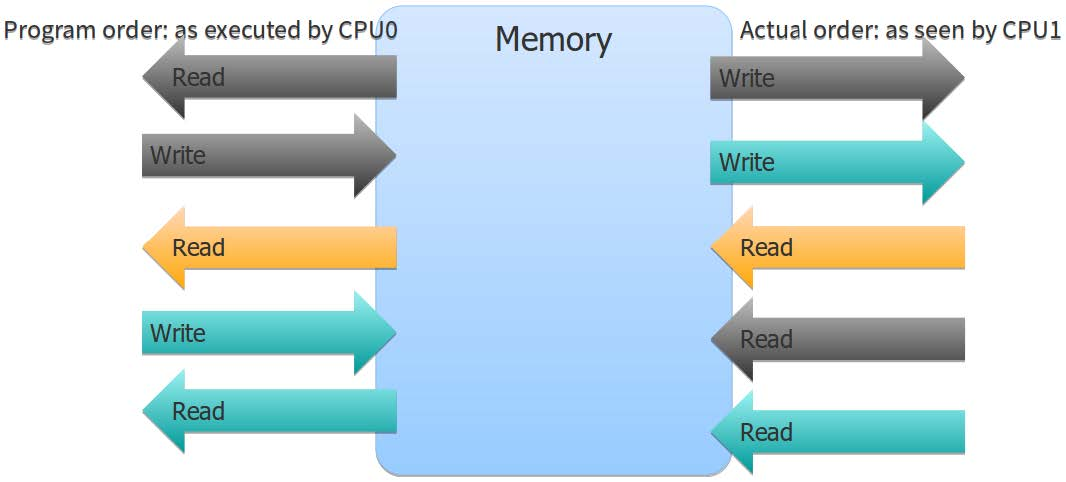
\includegraphics[width=0.6\textwidth]{content/1/chapter5/images/9.jpg}\\
圖5.9 - 自由內存序操作的可見性
\end{center}

這就是可見性,CPU按照一定的順序執行操作,但結果對其他CPU是可見的,但順序卻不同。這裡,我們通常只討論操作的可見性,而不是每次的結果。

在共享計數器\texttt{N}上的操作是按照自由內存序執行的,這會讓我們陷入嚴重的麻煩中。使程序正確的唯一方法是使用鎖,以便只有一個線程(生產者或消費者)運行,並且沒有從併發性方面得到性能的改進。

幸運的是,還可以使用其他的內存序,比如獲取-釋放內存序。當原子操作按照這個順序執行時,可以保證訪問內存,並在原子操作之前執行的操作,在另一個線程對同一原子變量執行原子操作之前是可見的。類似地,在原子操作之後執行的操作只有在對同一變量進行原子操作之後才可見。同樣,當討論操作的可見性時,是說結果對其他CPU可見。這在圖5.10中很明顯:在左邊,CPU0在執行的操作。在右邊,與CPU1看到的相同的操作。特別要注意的是,右邊有顯式的原子寫操作。但是CPU1不執行原子寫,它執行一個原子讀來查看CPU0執行的原子寫的結果。所有其他操作也一樣:左邊,是CPU0的執行順序。右邊,是CPU1可見的順序。

%\hspace*{\fill} \\ %插入空行
\begin{center}
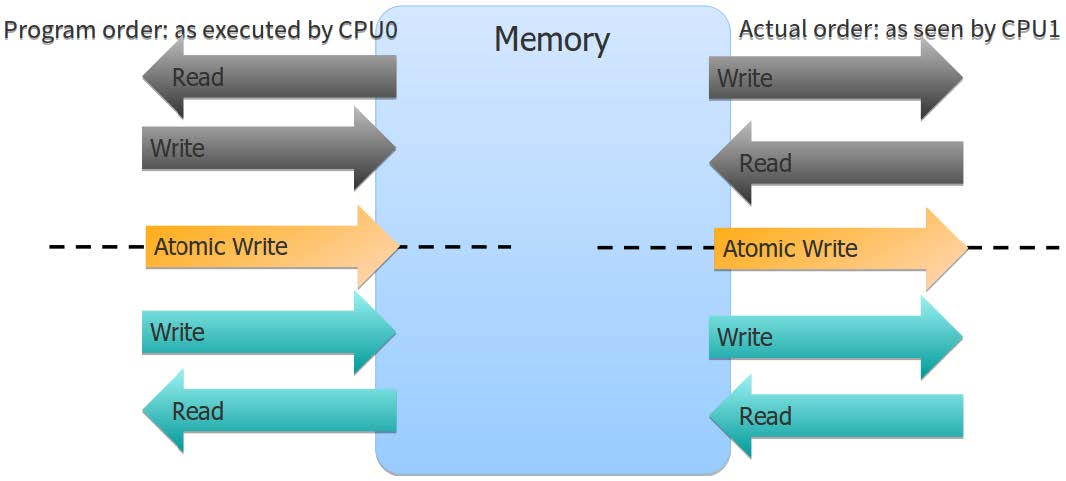
\includegraphics[width=0.6\textwidth]{content/1/chapter5/images/10.jpg}\\
圖5.10 - 獲取-釋放內存序操作的可見性
\end{center}

獲取-釋放是一個包含許多重要信息的聲明,這裡先來詳細闡述幾個不同的觀點。首先,順序是相對於兩個線程在同一個原子變量上執行的操作定義的。除非兩個線程以原子的方式訪問同一個變量,否則它們的時鐘對彼此來說完全沒意義,無法推斷出在其他事情前後發生了什麼。只有當一個線程觀察到另一個線程執行的原子操作的結果時,才可以在此基礎上,對操作前後的行為進行討論。在生產者-消費者的例子中,生產者以原子的方式增加計數器\texttt{N},消費者以原子的方式讀取同一個計數器。如果計數器沒有改變,則對生產者的狀態一無所知。但當消費者看到計數器從N變成了N+1,並且兩個線程都使用了獲取-釋放內存序,就知道生產者在計數器增加之前執行的所有操作,現在對消費者是可見的。這些操作包括構造相應的元素,並將其保存在數組\texttt{buffer[N]}中所需的所有工作,所以消費者可以安全地進行訪問。

第二個要點是,在訪問原子變量時,兩個線程都必須使用獲取-釋放內存序。如果生產者使用這個順序來增加計數值,但是消費者使用自由內存序來讀取,就不能保證操作的可見性了。

最後一點是,所有的順序都是根據對原子變量的操作前後給出的。同樣,在生產者-消費者的例子中,生產者為構造第N個對象而執行的操作結果,在消費者看到計數器變化時都是可見的。這些操作的可見順序沒有保證,可以在圖5.10中看到這一點。當然,在構建對象之前不能訪問,而當構建完成,就不關心完成的順序了。具有內存序的原子操作保證充當其他操作無法跨越的柵欄,可以在圖5.10中想象這樣存在這樣一個柵欄,它把整個程序分成兩個不同的部分:計數之前發生的和計數之後發生的操作。由於這個原因,討論類似內存柵欄這樣的原子操作通常會比較簡單。

假設,程序中計數器\texttt{N}上的所有原子操作都有獲取-釋放柵欄,這肯定能保證程序的正確性。然而,請注意,獲取-釋放對於我們的需求來說過度了。對於生產者來說,它給了我們保證,當消費者看到計數器從N到N+1的變化時,所有在計數增加到N+1之前構建的\texttt{buffer[0]}到\texttt{buffer[N]}都是可見的。還可以保證,為構造剩餘的對象、\texttt{buffer[N+1]}或更大的對象而執行的操作中,沒有一個是可見的。消費者不會訪問這些對象,直到它看到計數器的更新。在消費者端,保證在消費者看到計數器改變為N+1後,執行的所有操作都會在原子操作之後產生效果(內存訪問)。我們需要這樣的保證,不希望CPU重排消費者操作,並在準備好之前執行一些訪問對象\texttt{buffer[N]}的指令。但也可以保證消費者處理之前的對象(比如\texttt{buffer[N-1]})所做的工作已經完成,並且在消費者處理到下一個對象之前對所有線程可見。再說一遍,我們不需要這種保證,沒有任何操作需要這個保證。

嚴格的內存序是否有害?對正確性而言,沒有。但這是一本關於編寫高效程序(也是正確的程序)的書。為什麼內存序的保證是必須的呢?因為讓編譯器和處理器自己處理時,它們可以以重排程序的指令。為什麼要這麼做呢?通常是為了提高性能。因此,對重新排序執行的能力施加的限制越多,對性能越不利。因此,希望使用的內存序對程序的正確性有足夠的限制,但不能太嚴格。

為生產者-消費者程序提供所需要的內存序如下。在生產者端,需要獲得-釋放內存柵欄所提供的一半保證。所有在使用柵欄的原子操作之前執行的操作,必須在其他線程執行相應的原子操作之前可見。這就是釋放內存序:

%\hspace*{\fill} \\ %插入空行
\begin{center}
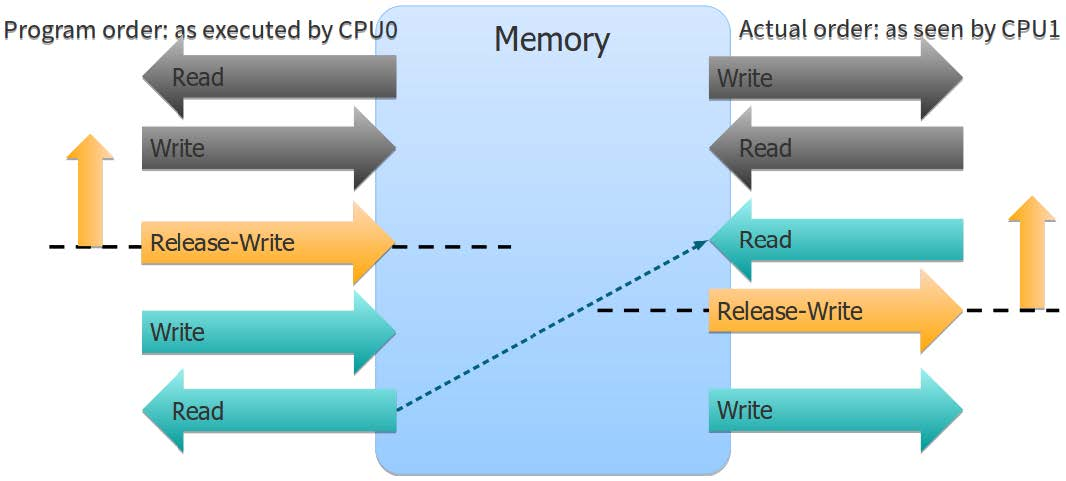
\includegraphics[width=0.6\textwidth]{content/1/chapter5/images/11.jpg}\\
圖5.11 - 釋放內存序
\end{center}

當CPU1看到CPU0以釋放內存序執行的原子寫操作結果時,可以保證CPU1看到的內存狀態已經反映給CPU0在這個原子操作之前執行的所有操作。注意,沒有提到CPU0在原子操作之後執行的操作。正如在圖5.11中看到的,這些操作可以以任何順序顯示。由原子操作創建的內存柵欄只在一個方向上有效。在柵欄之前執行的操作都不能跨越它,並且在柵欄之後才看到。但是在另一個方向上,柵欄是可滲透的。出於這個原因,釋放內存柵欄和相應的獲取內存柵欄有時稱為\textbf{半柵欄}。

獲取內存序在消費者端使用,確保柵欄後執行的所有操作對柵欄後的其他線程可見,如圖5.12所示:

%\hspace*{\fill} \\ %插入空行
\begin{center}
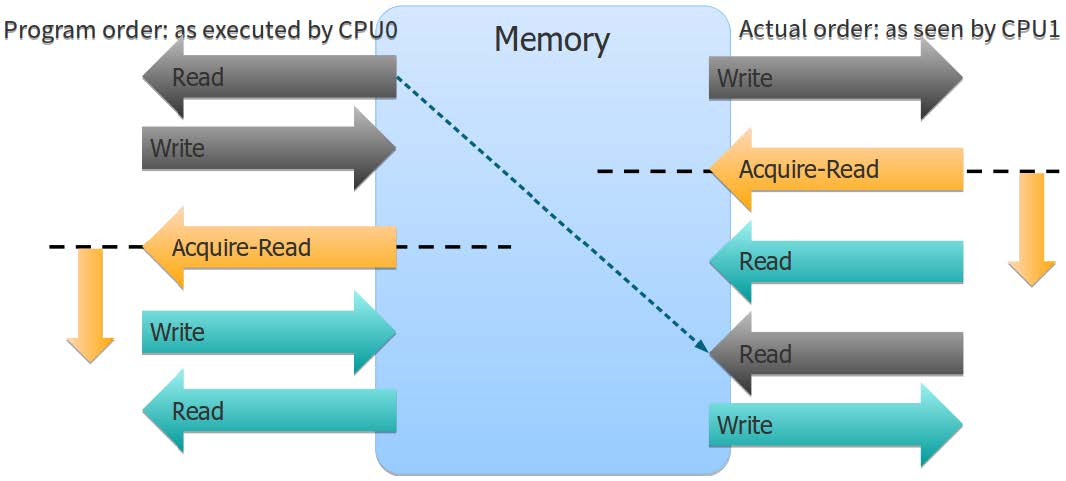
\includegraphics[width=0.6\textwidth]{content/1/chapter5/images/12.jpg}\\
圖5.12 - 獲取內存序
\end{center}

獲取和釋放內存柵欄總是成對使用:如果一個線程(在我們的例子中,是生產者線程)使用一個原子操作來釋放內存,那麼另一個線程(消費者線程)必須在同一個原子變量上使用獲取內存序。為什麼需要兩個柵欄?一方面,可以保證生產者在增加計數之前構建新對象所做的一切,只要看到這個增量,消費者就可以看到。但這還不夠,因此需要保證消費者為處理這個新對象而執行的操作不會在時間上向後移動,回到柵欄之前的某個時刻,此時他們可能已經看到了處於未完成狀態的對象。

僅僅對共享數據進行原子化操作是不夠的,上面的方法對生產者-消費者項目是否真的有效?鎖和無鎖版本都是正確的,儘管沒有明確地說明內存序。那麼,C++是如何控制內存序的呢?

\subsubsubsection{5.5.3\hspace{0.2cm}C++中的內存序}

首先,回想一下我們的生產者-消費者程序的無鎖版本,那個有原子計數器的版本:

\begin{lstlisting}[style=styleCXX]
std::atomic<size_t> N; // Count of initialized objects
T* buffer; // Only [0]…[N-1] are initialized
… Producer …
{
	new (buffer + N) T( … arguments … );
	++N; // Atomic, no need for locks
}
… Consumer …
for (size_t i = 0; keep_consuming(); ++i) {
	while (N <= i) {}; // Atomic read
	consume(buffer[i]);
}
\end{lstlisting}

計數器\texttt{N}是一個原子變量,由模板\texttt{std::atomic}生成的類型對象,類型參數為\texttt{size\_t}。所有原子類型都支持原子讀寫操作,可以出現在賦值操作中。此外,整數原子具有以原子方式定義和實現的常規整數操作,因此\texttt{++N}是一個原子增量(並不是所有操作都定義了,例如:沒有\texttt{operator *=})。這些操作都沒有明確指定內存序,那麼如何保證內存序呢?在默認情況下,內存序會得到最嚴格的保證,即每個原子操作的雙向內存柵欄(實際的保證甚至更加嚴格,將在下一節中看到)。這就是我們的程序正確的原因。

若認為這有些過度了,那可以將內存序改為所需要的,但必須顯式地進行。原子操作也可以通過調用\texttt{std::atomic}類型的成員函數來執行,在這裡也可以指定內存順序。用戶線程需要使用獲取柵欄進行加載操作:

\begin{lstlisting}[style=styleCXX]
while (N.load(std::memory_order_acquire) <= i);
\end{lstlisting}

生產者線程需要一個帶有釋放柵欄的自增操作(就像自增操作符一樣,成員函數也會返回自增操作完成之前的值):

\begin{lstlisting}[style=styleCXX]
N.fetch_add(1, std::memory_order_release);
\end{lstlisting}

在優化過程中,已經跳過了一個非常重要的步驟。如果認為這有些過度了,那麼必須通過性能測試來證明,只有這樣才能將保證達到性能和正確性的真正平衡。即使在使用鎖的情況下,併發程序也很難編寫,必須證明無鎖代碼和內存序的正確性。

鎖的內存順序是什麼呢?鎖保護的操作都將被隨後獲得鎖的任何其他線程看到,但是剩下的內存呢?使用鎖所強制的內存序如圖5.13所示:

%\hspace*{\fill} \\ %插入空行
\begin{center}
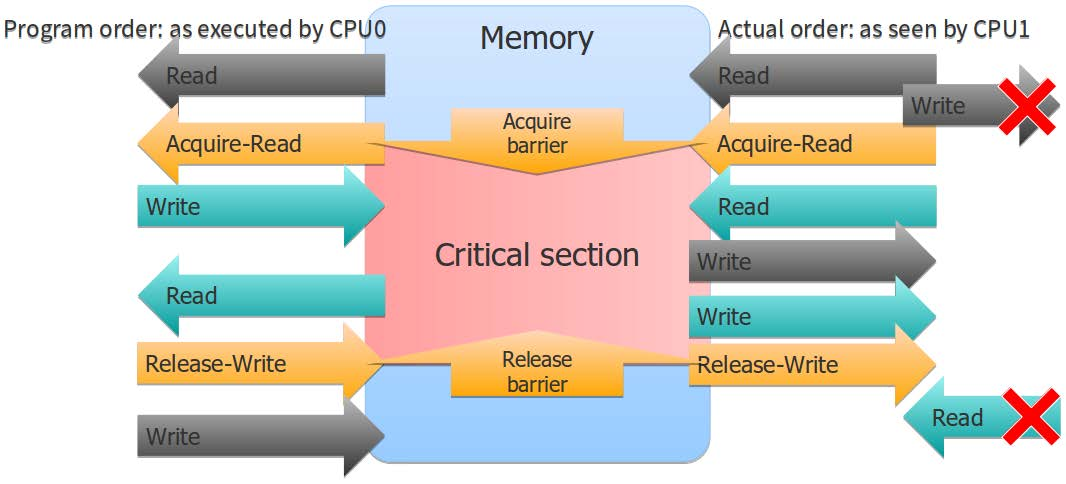
\includegraphics[width=0.6\textwidth]{content/1/chapter5/images/13.jpg}\\
圖5.13 - 互斥鎖的內存序
\end{center}

互斥對象內部(至少)有兩個原子操作。鎖定互斥鎖相當於讀取操作和獲取內存序(這解釋了獲取鎖時使用的內存序)。在柵欄前執行的操作,都可以在越過柵欄後看到,但是在獲得鎖之後執行的操作都不能在之前看到。解鎖或釋放鎖時,即為釋放內存序。在柵欄之前執行的操作將在柵欄之前可見,獲取和釋放這對柵欄充當了夾在它們之間的邊界,這就是所謂的臨界區。在臨界區內執行的操作,在線程持有鎖時執行的操作,在進入臨界區時對其他線程都是可見的。操作都不能離開臨界區(在之前或之後變得可見),但是外部的操作可以進入臨界區。至關重要的是,沒有操作可以跨越臨界區。如果外部操作進入臨界區,就不能離開。因此,CPU0在進入臨界區之前所做的事情,都會在離開臨界區之後讓CPU1可見。

對於我們的生產者-消費者計劃,這會轉化為以下保證:

\begin{lstlisting}[style=styleCXX]
… Producer …
new (buffer + N) T( … arguments … );
{ // Critical section start – acquire lock
	std::lock_guard l(mN);
	++N;
} // Critical section end - Release lock
… Consumer …
{ // Critical section – acquire lock
std::lock_guard l(mN);
n = N;
} // Critical section – release lock
consume(buffer[N]);
\end{lstlisting}

生產者為構造第N個對象而執行的所有操作,都在生產者進入臨界區之前完成。將在消費者離開臨界區時,開始使用第N個對象之前對其可見。因此,程序是正確的。

剛才的部分介紹了內存序的概念,並舉例進行了說明。但是,當試圖在代碼中使用這些知識時,會發現結果不一致。為了更好地理解性能,應該從同步多線程和避免數據競爭的不同方法中期望得到什麼,所以需要一種稍微複雜的方式來描述內存序和相關概念。




































